\section{Evaluation}\label{sec:evaluation}

The evaluation of our preemption point placement algorithm will embody
two methods: 1) characterization and measurement of preemption costs
using real-time application code, and 2) a breakdown utilization schedulability
comparison for various CRPD computational approaches.
%2) a schedulability comparison
%of synthetic task set for various preemption models.

\subsection {Preemption Cost
  Characterization}\label{sec:preemption_cost_measurement}
To characterize the behavior and estimate the benefit of the approach
proposed in this paper, a case study of representative tasks was
performed. The tasks were selected from Malardalen University of
Sweden's WCET benchmark suite~\cite{mrtc:01}. Each task was built using Gaisler's
Bare-C Cross Compiler~\cite{gaisler:01} for the GRSIM
LEON3~\cite{gaisler:02} simulated target.

Within a task, variance in the number of shared UCBs between program
points is related to the execution flow of the task through each of
the points. For instance, one path to ${P_j}$ may include only ${P_h}$,
while another path to ${P_j}$ may contain ${P_h}$ followed by
${P_i}$. The set of UCBs shared between ${P_h}$ and ${P_j}$ may differ
based on the path between them. If the paths differ one of them may
result in a greater number of shared UCBs between the points. To
accurately upper-bound the shared UCBs between points requires
complete control flow information.

Tasks were first analyzed using AbsInt's a\textsuperscript{3} WCET~\cite{absint:01}
to determine the set of basic blocks. Next, the basic
blocks ${\{B_1, B_2, ..., B_n\}}$ were serialized by recording their
order during execution. Program points ${\{P_1, P_2, ..., P_n\}}$ were
assigned by setting ${P_i}$ to the address of the final instruction of
each basic block ${B_i}$ for ${i}$ from ${0}$ to ${n}$.

Each program point ${P_j}$ served as a breakpoint when running the
task on the simulator. As the task was executed, at each breakpoint
${P_j}$, the instruction and data cache states were saved as ${I_j}$
and ${D_j}$. Given the limitations of the simulator and
a\textsuperscript{3} it was not possible record the actual control
flow. Thus, calculating an accurate over-estimate of the UCBs shared
between program points was not possible. A selection of cache
snapshots were chosen to representation the actual behavior.

The representative cache contents were selected as the final visit of
each program point. A program point ${P_i}$ may be visited multiple
times during a tasks execution. The UCBs shared between ${P_i}$ and a
later point ${P_j}$ could change with each visit of ${P_i}$. During
the final visit of ${P_i}$ the instruction and data cache contents
were captured, and recorded as ${I_i}$ and ${D_i}$. From these
representative snapshots, a representative over-estimate of shared
UCBs were made.

Shared UCBs were calculated by intersecting the cache state from ${P_i}$
to ${P_j}$, except ${P_j}$. A cache line that remains unchanged after
the execution of ${\langle}$ ${P_i}$, ${P_{i+1}}$, ..., ${P_{j-1}}$
${\rangle}$ will be
present in the cache before execution of the basic block that ${P_j}$
represents. It is only from these unchanged cache lines that the shared UCBs
between ${P_i}$ and ${P_j}$ can be selected. The complete set of
unchanged cache lines serves as a safe upper-bound on the shared UCBs
between the two points. The equation below formalizes this idea, using
${H}$ as either the set of instruction cache or data cache snapshots.
\vspace{-20pt}
\begin{center}
  \begin{equation*}
    UCB(P_i, P_j) = \bigcap_{k=i}^{j-1} H_k
  \end{equation*}
\end{center}

\subsubsection{Availability}

This method may be verified and reproduced using the same tools and
data. Gaisler's compiler and simulator are freely available. AbsInt's
a\textsuperscript{3} tool is available for educational and evaluation
purposes. The programs written and data used in this paper can be
found on GitHub~\cite{tessler:14} thereby permitting the research community
to reproduce and leverage our work as needed.

\subsubsection{Results}

The results are presented as a comparison between the our proposed
method and the Bertogna approach. For a program point ${P_j}$ the
Bertogna \cite{bertogna:11} approach defines the UCBs (and therefor the CRPD) as:
\begin{equation*}
  \max\{ UCB(P_i, P_j) \vert i < j \}
\end{equation*}

To determine the maximum benefit of the new approach, the best case
scenario is considered. When the preemption point is selected with the
fewest number of UCBs based upon previous preemption.  For ${P_j}$ the
determination is made by:
\begin{equation*}
  \min\{ UCB(P_i, P_j) \vert i < j \}
\end{equation*}

In the following graphs, each point in the graph represents two points
in the program. The first point of the program ${P_i}$ is fixed by the
x-axis. The y-axis indicates the shared UCB count with a later program
point. The first graph, which represents the recursion benchmark's
data cache, is for illustration. At program point four, the Bertogna
approach finds 24 shared UCBs between point four and point five. The
proposed method selects program point seven with a shared UCB count of
14.
%
\begin{figure}[h!]
\vspace{-10pt}
\begin{center}
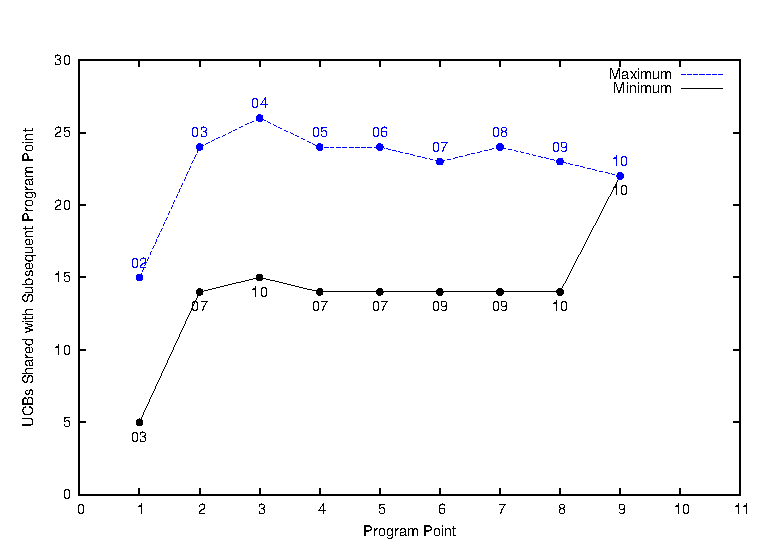
\includegraphics[width=\linewidth]{eps/recursion-dcache.eps}
\caption{Recursion Data Cache.}
\label{fig:recusion_data_cache}
\end{center}
\vspace{-20pt}
\end{figure}
To compare the two approaches their selection of two program points is
simulated by assuming ${Q}$ is larger than the task's total execution
time. Bertogna's approach would select the lowest value of the
dashed line. The proposed approach would select the lowest value of
the solid line. The difference between these two UCB counts is the
benefit provided by the proposed approach.
\begin{figure}[h!]
\vspace{-10pt}
\begin{center}
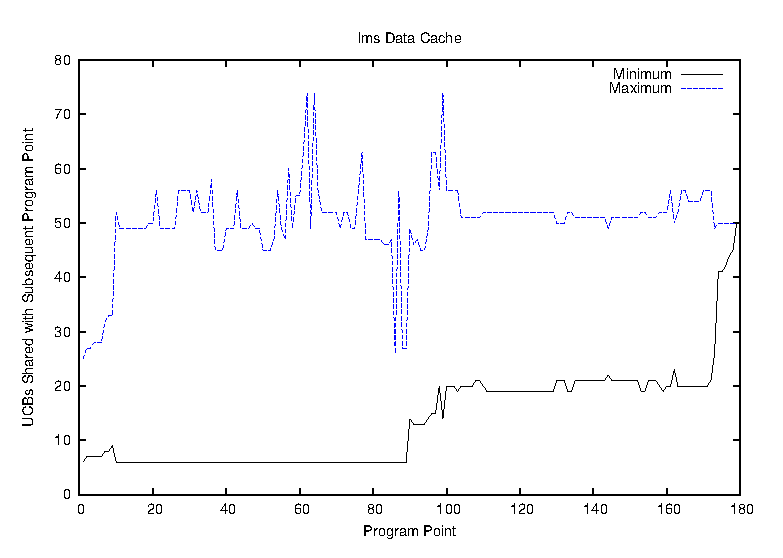
\includegraphics[width=\linewidth]{eps/lms-dcache.eps}
\caption{LMS Data Cache.}
\label{fig:lms_data_cache}
\end{center}
\end{figure}
%
\begin{figure}[h!]
\vspace{-20pt}
\begin{center}
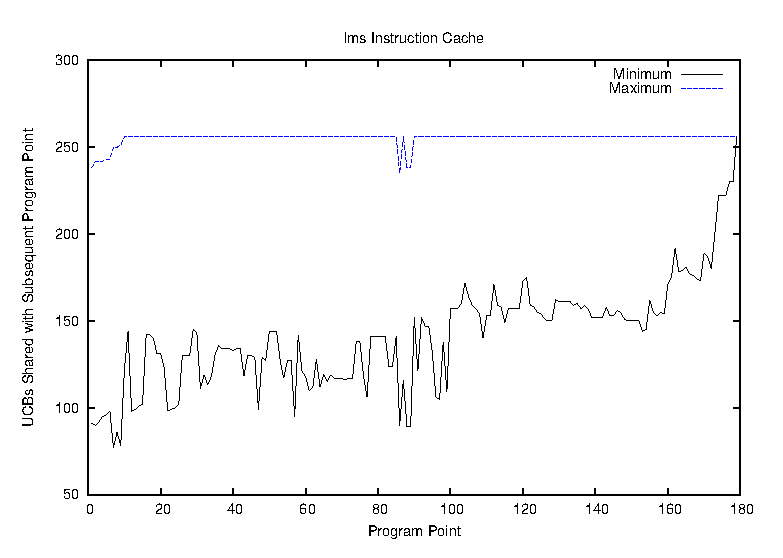
\includegraphics[width=\linewidth]{eps/lms-icache.eps}
\caption{LMS Instruction Cache.}
\label{fig:lms_instruction_cache}
\end{center}
\vspace{-10pt}
\end{figure}
%
\begin{table}[h!]
%{\fontsize{10}{10}\selectfont
\small
\begin{minipage}{\linewidth}
\centering
    \begin{tabular}{l | l | l || l | l | l}
      Task & Cache & Benefit & Task & Cache & Benefit\\
      \hline

      adpcm & ${I}$ & 143 & fft1 & ${I}$ & 72 \\
            & ${D}$ & 5 & & ${D}$ & 13\\
      \hline

      bsort & ${I}$ & 0 & fibcall & ${I}$ & 1 \\
            & ${D}$ & 0 & & ${D}$ & 1 \\
      \hline

      cnt & ${I}$ & 63 & lms & ${I}$ & 158 \\
          & ${D}$ & 2 & & ${D}$ & 18 \\
      \hline

      cover & ${I}$ & 135 & ndes & ${I}$ & 96 \\
            & ${D}$ & 2 & & ${D}$ & 15 \\
      \hline

      crc & ${I}$ & 18 & recursion & ${I}$ & 7 \\
          & ${D}$ & 1 & & ${D}$ & 10  \\
      \hline

    \end{tabular}
    \bigskip
    \caption {Benefit of Proposed Method}
    \label{tab:proposed_method_benefit}
%
%    Benefit of Proposed Method
%    \bigskip
\end{minipage}
\normalsize
%}
\vspace{-20pt}
\end{table}
%
%\begin{minipage}{\linewidth}
%\centering
%  \caption {Benefit of Proposed Method}
%    \begin{tabular}{l l | l}
%      Task & Cache & Benefit \\
%      \hline
%
%      adpcm & ${I}$ & 143 \\
%            & ${D}$ & 5 \\
%      \hline
%
%      bsort & ${I}$ & 0 \\
%            & ${D}$ & 0 \\
%      \hline
%
%      cnt & ${I}$ & 63 \\
%          & ${D}$ & 2 \\
%      \hline
%
%      cover & ${I}$ & 135 \\
%            & ${D}$ & 2 \\
%      \hline
%
%      crc & ${I}$ & 18 \\
%          & ${D}$ & 1 \\
%      \hline
%
%      fft1 & ${I}$ & 72 \\
%           & ${D}$ & 13 \\
%      \hline
%
%      fibcall & ${I}$ & 1 \\
%              & ${D}$ & 1 \\
%      \hline
%
%      lms & ${I}$ & 158 \\
%          & ${D}$ & 18 \\
%      \hline
%
%      ndes & ${I}$ & 96 \\
%           & ${D}$ & 15 \\
%      \hline
%
%      recursion & ${I}$ & 7 \\
%                & ${D}$ & 10 \\
%      \hline
%
%    \end{tabular}
%    \bigskip
%
%    Benefit of Proposed Method
%    \bigskip
%\end{minipage}
%
Examining the graphs for all tasks and caches (instruction and data)
there are a few common traits. The minimum shared UCBs sharply
increases at the end of the tasks execution. This is due to the nature
of the over-estimation of shared UCBs and the tasks, the number of
instructions in the basic block between the final program points is
relatively small; limiting the number of cache lines that could be
filtered by the intersection.

This behavior limits the appropriate type of analysis. The preceding
table shows the maximum benefit of the proposed approach. If the
minimum benefit were considered it would always be zero; since the
difference in estimated shared UCBs converges at the final basic
block.

Drastic spikes downwards in the shared UCB counts for the minimum and
maximum approaches coincide with function call boundaries, or large
conditional blocks. At these boundaries, the maximum and minimum
approaches have similar UCB counts. This may be an area for further
study, using a greater number of tasks.

There is a sharp upward spike in the early program points for the
maximum approach. This is likely due to the early initialization
blocks built into tasks. The minimum approach shows a clear benefit of
selecting a preemption point outside of the early initialization
section.
\subsection{Breakdown Utilization}

The previous analysis illustrates the benefit of the proposed
approach for an individual task, which does not illustrate the
schedulability benefit. To determine the schedulability benefit a
second case study was performed. Focusing on the breakdown utilization
when comparing the UCB only approach for EDF~\cite{lunniss:13}. For
convenience the UCB Only approach for EDF will be referred to as
${UOE}$, and Explicit Preemption Point Placement as ${EPP}$.

The appropriate schedulablity test for ${UOE}$ is found in
Lunniss \emph{et~al.}~\cite{lunniss:13}. It is comprised of three
parts: ${\gamma^{ucb}_j}$, ${U^*_j}$, and ${U^*}$. They represent
the maximum CRPD for a task ${j}$, the utilization of the task ${j}$
including the CRPD of the task, and the utilization of the task set.
A task set is schedulable when ${U^* \le 1}$.
\begin{equation}
  \gamma^{ucb}_j = BRT \cdot \max\limits_{k \in \tau}
  \left\{ \left| UCB_k \right| \right\}
\end{equation}
\begin{equation}
  U^*_j = \frac{C_j + \gamma^{ucb}_j}{T_j}
\end{equation}
\begin{equation}
  U^* = \sum_{i \in \tau} U^*_i
\end{equation}

The task set from which the breakdown utilization benefit is
calculated comes, again, from the MRTC suite \cite{mrtc:01}. Borrowing
the technique from \cite{lunniss:13}, each task has its deadline (and
therefor period) set to ${T_i = u \cdot C_i}$
where ${u}$ is a constant. The constant, ${u}$, begins at the number
of tasks (ten) and is increased in steps of .25 until the task set
becomes schedulable. Incremental negative adjustments are then made to
determine when the set becomes unschedulable, indicating the breakdown
utilization.

The final parameter, ${UCB_k}$ is obtained by modifying the earlier
evaluation section \emph{Preemption Cost Characterization}. For each
task, the set of shared UCBs are calculated at each program
point. Taking the maximum shared UCB count as ${UCB_k}$ for any task
is safe and appropriate for calculating ${U^*}$.Similarly, for ${EPP}$,
the shared UCB counts obtained in the earlier evaluation serve as input for
the Explicit Preemption Point algorithm.  The last input variables required
for both approaches are ${C_i}$ and ${BRT}$. ${C_i}$ was captured as the
total number of cycles required to complete the task without preemptions.
The ${BRT}$ is set to 7.8 ${{\mu}s}$, the refresh time of main memory.

The breakdown utilization determination leverages our iterative schedulability
and preemption point placement algorithm as outlined in the following steps below
as given in Algorithm~\ref{alg:iterative-breakdown-utilization-algo}.
%{\fontsize{10}{10}\selectfont
\begin{algorithm}
\caption{Iterative Breakdown Utilization Evaluation Algorithm}
\label{alg:iterative-breakdown-utilization-algo}
\begin{algorithmic}[1]
\small
\State{Start with a task system that may or may not be feasible.}
\State{Assume the CRPD of the task system is initially zero.}
\Repeat
   \State\begin{varwidth}[t]{\linewidth}
    Run the Iterative Schedulability and Preemption Point Placement Algorithm \ref{alg:iterative-schedulability-optimal-ppp} \par
    \end{varwidth}
%
%    \Repeat
%        \State\begin{varwidth}[t]{\linewidth}
%        Run the Baruah algorithm to obtain the maximum \par
%        \hskip\algorithmicindent non-preemptive region $Q_i$ for each task.
%        \end{varwidth}
%        \State\begin{varwidth}[t]{\linewidth}
%        Select optimal preemption points using our \par
%        \hskip\algorithmicindent dynamic programming algorithm.
%        \end{varwidth}
%        \State\begin{varwidth}[t]{\linewidth}
%        Compute the CRPD and the preemptive WCET \par
%        \hskip\algorithmicindent $C_i$ from the selected preemption points.
%        \end{varwidth}
%    \Until{the selected preemption points do not change.}
%
    \If{the task system is feasible/schedulable}
        \State\begin{varwidth}[t]{\linewidth}
        Increase the system utilization by decreasing the \par
        \hskip\algorithmicindent periods via a binary search.
        \end{varwidth}
    \Else
        \State\begin{varwidth}[t]{\linewidth}
        Decrease the system utilization by increasing the \par
        \hskip\algorithmicindent periods via a binary search.
        \end{varwidth}
    \EndIf
\Until\begin{varwidth}[t]{\linewidth}
the utilization change is less than some tolerance.
\end{varwidth}
\State{The breakdown utilization is given by U.}
\normalsize
\end{algorithmic}
\end{algorithm}
%}
Using ten tasks, the breakdown utilization comparison between ${UOE}$
and ${EPP}$ are summarized in the table below.
\begin{table}[h!]
\small
\begin{minipage}{\linewidth}
\vspace{-20pt}
  \bigskip
  \centering
    \begin{tabular}{c | c}
      Method & Utilization \\
      \hline
      UOE & .29 \\
      EPP & TBD \\
    \end{tabular}
    \bigskip
    \caption {Breakdown Utilization Summary}
    \label{tab:breakdown_utilization_summary}
\normalsize
\end{minipage}
\normalsize
%\vspace{-20pt}
\end{table}
Compared to \cite{lunniss:13} this evaluation of ${UOE}$ has a
breakdown utilization 17\% lower. This is likely due to the
(differing) selection of tasks and estimation of UCBs. The data used
in \cite{lunniss:13} does not include UCB information per basic block,
which is required for ${EPP}$. Necessitating the generation of new
UCB estimations per task.
%
%\clearpage
%
%\subsection {Taskset Schedulability Evaluation}\label{sec:taskset schedulability}
%The schedulability performance metrics we intend to compare various
%preemption models with are: 1) the percentage of schedulable task sets
%as a function of the task set utilization, 2) the percentage of
%schedulable task sets as a function of the number of tasks, 3) the
%percentage of schedulable task sets as a function of the maximum CRPD,
%and 4) the percentage of schedulable task sets as a function of the
%variability of the CRPD variance \begin{math}\sigma_{CRPD}\end{math}.
%The following preemption models will be studied namely: 1) fully
%non-preemptive, 2) fully preemptive, 3) limited preemption naive
%approach, 4) limited preemption point placement with fixed CRPD
%preemption cost, 5) limited preemption point placement with variable
%CRPD preemption cost, and 6) optimal preemption point placement with
%enhanced CRPD preemption cost.
%
%Our approach for generating the synthetic task sets involves a number
%of steps which is summarized as follows.  The number of basic blocks
%generated each task is in the
%interval \begin{math}[N_{i}(min),N_{i}(max)]\end{math} using a random
%uniform distribution.  Each basic block non-preemptive WCET is
%generated using a Gaussian distribution with
%mean \begin{math}\mu_{WCET}\end{math} and
%variance \begin{math}\sigma_{WCET}\end{math}.  The  utilization of
%each task has been generated using the approach proposed in [TBD12].
%The task periods \begin{math}T_{i}\end{math} were then computed
%dividing the non-preemptive WCET \begin{math}C_{i}^{NP}\end{math} by
%the utilization \begin{math}U_{i}\end{math} of each task.  Preemption
%costs were randomly generated using the following function (TBD), to
%achieve a realistic distribution similar to the one derived
%empirically).  The enhanced CRPD is generated to be a percentage of
%the WCET in the interval [0, 0.50] with a random uniform
%distribution. Cache related preemption delay (CRPD) values are
%generated for each pair of potential preemption points.  The variable
%CRPD preemption cost model uses the CRPD cost from the each preemption
%point to the end of the task. The fixed CRPD preemption cost model
%uses the maximum CRPD cost of all variable CRPD preemption cost
%values.
